% Chapter4
\chapter{Implementierung} \label{chapter:thevetestcase}
\section{Modellierung der Anlage}
\section{Aufbau der Anlage}
\section{Phasen und Rezepte}
\section{HMI}
Für dieses Projekt wurde als SCADA System die Software zenon vorgegeben, daher wurde das HMI in zenon Supervisor (zenons HMI Programm) umgesetzt.\\
\\
\textbf{Visualisierung}\\
In zenon wird eine Visualisierung  \glqq Bild\grqq\space  gennant. Dieses kann man mit vorgefertigten Elementen erweitert werden. 

Als Ausgangspunkt für die Visualisierung wurde das RI-Fließeschema zur Hand genommen. Von diesem wurde die Anzahl der Elemente und die Grundstruktur übernommen. Als nächsten Schritt musste evaluiert werden, welche Inhalte des RI-Fließschemas für die Visualisierung relevant und welche Informationen nicht vorhanden waren.
\begin{description}
\item[Wichtige Elemente]~\par
	\begin{itemize}
		\item Rohre in Verwendung kennzeichnen
		\item Sensorwerte anzeigen
		\item ....ADD MORE
	\end{itemize}
\end{description}
%todo add image
ABBILDUNG\\

\textbf{Feldbuskonfiguration}\\
Um eine Visualisierung mit aktuellen Sensorwerten zu befüllen, wird eine Verbindung zur SPS benötigt. In zenon wird eine Verbindung über zenon Logic (im weiteren nur noch Logic genannt) hergestellt.\\
\\
Als ersten Schritt, um in Logic eine SPS hinzuzufügen, musste im Unterpunkt \glqq Feldbuskonfiguration\grqq\space die Treibersoftware für die ADAM5550 SPS hinzugefügt werden. Darauf hin wurden alle Module, die an der SPS angebracht wurden, in dieser Konfiguration hinzugefügt.\\%todo Position
\begin{figure}[h!]
  \centering
  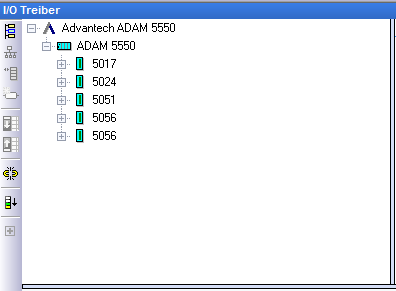
\includegraphics[width=0.7\textwidth]{graphics/implementation/Feldbuskonfiguration}
  \caption{Feldbuskonfiguration}%todo Grafik name
\end{figure}
\\
\textbf{Variablen}\\
In zenon können auf mehrere Arten Variablen erstellt werden, damit diese jedoch für die Visualisierung und von Logic sichtbar sind, müssen sie als Globale Variable definiert werden. Der einfachste Weg dafür ist es, im Logic Variablenfenster über den Reiter  \glqq Globale Variablen\grqq\space  die Funktion  \glqq Variable hinzufügen\grqq\space  aufzurufen.\\%todo Position
\begin{figure}[h!]
  \centering
  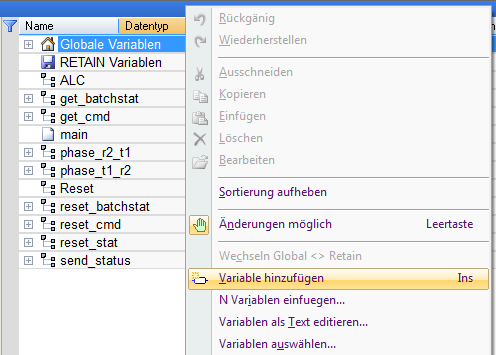
\includegraphics[width=0.7\textwidth]{graphics/implementation/Variablen}
  \caption{Variablen}%todo Grafik name
\end{figure}\\
Nachdem alle Variablen erstellt wurden, müssen diese mit der Feldbuskonfiguration verknüpft werden. Durch diesen Schritt erhält man Zugang zu den an der SPS angeschlossenen Elementen.\\
Die erstellten Variablen mussten als nächstes in der Visualisierung eingetragen werden um in dieser im nächsten Schritt eine Steuerung zu erzeugen.\\
\\
%Feldbuskonfiguration -> Konfiguration einfügen (Advantech ADAM 5550) -> Master/Port hinzufügen (ADAM 5550) -> Slave/Datenblock einfügen (Slot:Steckplatz an SPS; Module: Analog/Digital|In/Out|4/8/16 Channels...) -> Variable hinzufügen (Channel; Variablenname)
%Variable -> Globale Variable hinzufügen (erzeugt Variable in logic und auch im supervisor zugänglich für die Visualisierung) -> In Visualisierung zu den Elemente die richtigen Variablen hinzufügen -> Bei Feldbbuskonfiguration bei richtiger I/O auf richtigem Channel hinzufügen
%TEST -> logic Programm hochladen -> Variablen in logic zeigen aktuelle werte an -> check mit werten direkt von der SPS

%Umrechnen von Sensorwerten: 
%Durchflusssensor Digital -> etwa 900 ticks pro Liter -> Timer bid 900 ticks -> Liter/min
%Füllstandsensor 4-20mA -> 4=voll, 20=leer -> Variablen/Tank Konfiguration -> Umrechnung 4=100, 20=0
%Ventilstatus 0/1 -> Variablen Konfiguration -> Extremwerte farblich markieren -> Ventil Elementfarbe nach Variablen Farbe
\textbf{Steuerung}\\
Phase 1 Steuerung mittels Buttons\\
	Der erste Versuch war es die Steuerung mittels einfachen Buttons umzusetzen. Diese haben meist die in zenon vorhandene Funktion  \glqq Sollwert absetzen\grqq\space  verwendet, welche den Wert einer Variable ändert.\\
	So konnten alle Funktionen umgesetzt werden, dadurch erhielt das  \glqq Bild\grqq\space  jedoch viele Elemente die von der Eigentlichen Visualisierung ablenkten.\\
\\
Phase 2 Versteckte Buttons\\
	Um den Element-Overload zu verringern war der nächste Schritt die Button zu  \glqq verstecken\grqq\space  indem sie Transparent über die eigentlichen Elementen (beispielsweise ein Ventil) verschoben wurden.\\
	In der Visualisierung wurden nun weniger  \glqq unwichtige\grqq\space  Bausteine angezeigt, die Elemente waren jedoch immer noch da, wodurch die Größe (MB) der Visualisierung deutlich anstieg.\\
\\
Phase 3 Funktionale Elemente\\
	Der nächste schritt war es die nicht funktionalen Grafikelemente durch Buttons in Form der gewünschten Elemente zu ersetzten.\\
\\
\textbf{Rezepterstellung}\\

\section{Ontology}
\section{Aktivitätsdiagramm}
\section{Codegenerierung}

TODO